\section{Gradient Descent Algorithm}\label{sec: GD}
\subsection{Gradient Descent}
Gradient descent is part of a family of algorithms called descent methods. With descent methods a minimizing sequence $(x^{(k)})$ with $k = 1,\ldots$ can be generated where $$x^{(k+1)} = x^{(k)} + \tau^{(k)} \Delta x^{(k)}$$ Here $\tau^{(k)} > 0$ is called the step size and $\Delta x^{(k)}$ is called the search direction. The superscripts $k=0,1\ldots$ denote the iteration numbers. Since the goal is to eventually minimize the function $f$ in \eqref{eq:8}, it should hold that $f(x^{(k+1)}) < f(x^{(k)})$ for every $k \in \mathbb{N}$ considered, until an optimal solution is reached. To achieve a decrease in the function value in every iteration, the search direction needs to satisfy the following strict inequality: $$\nabla f(x^{(k)})^{T} \Delta x^{(k)} < 0.$$ By definition, the gradient of the function at the current iteration, say $\nabla f(x^{(k)})$, points in the direction of the steepest increase of the function. To minimize $f$, the search direction $\Delta x^{(k)}$ should be chosen to point in the opposite direction. This means that the angle between the gradient and the search direction should be acute, and as a result, the inner product between $\nabla f(x^{(k)})$ and $\Delta x^{(k)}$ should be less than 0. As stated in \cite[464]{boyd2004convex}, a general descent method consists of the following stages: 
\begin{algorithm}
\caption{\textit{General descent method}}
\begin{algorithmic}
\State \textbf{Given} a starting point $x \in \textbf{dom} (f)$.
\vspace{0.03cm}
\State \textbf{repeat}\\
\begin{enumerate}
    \item Determine a descent direction $\Delta x.$
    \item \textit{Line search.} Choose a step size $\tau > 0$.
    \item \textit{Update.} $x := x + \tau \Delta x.$
\end{enumerate}
\State \textbf{until} stopping criterion is satisfied.
\end{algorithmic}
\end{algorithm}\\
The negative gradient $\Delta x = -\nabla f(x)$ is a natural choice for the search direction. The resulting algorithm is called the \textit{gradient descent method.} As stated in \cite[466]{boyd2004convex}, the gradient descent method consists of the following stages:
\begin{algorithm}
\caption{\textit{Gradient descent method}}\label{Pseudocode_GD}
\begin{algorithmic}
\State \textbf{Given} a starting point $x \in \textbf{dom} (f)$.
\vspace{0.03cm}
\State \textbf{repeat}\\
\begin{enumerate}
    \item $\Delta x := -\nabla f(x).$
    \item \textit{Line search.} Choose a step size $\tau > 0.$
    \item \textit{Update.} $x := x + \tau \Delta x.$
\end{enumerate}
\State \textbf{until} stopping criterion is satisfied.
\end{algorithmic}
\end{algorithm}\\
The second step in the repeat block is known as the \textit{line search}. The step size $\tau$ determines the next vector $x$. We consider two approaches for determining the step size, namely fixed step size and line search. In the fixed step size method, the same step size $\tau$ is used for every iteration until the stopping criterion is met. On the other hand, the line search method adjusts the step size at each iteration to ensure that the algorithm progresses toward the minimum without overshooting it. Specifically, the line search method searches for the optimal step size that minimizes the cost function along the descent direction. This allows the algorithm to take larger steps when the slope is steep and smaller steps when the slope is flat. The stopping criterion is often checked immediately after the descent direction $\Delta x$ is computed. The stopping criterion is of the form $||\nabla f(x)||_{2} \leq \eta,$ where $\eta$ is small and positive. 

\subsection{Convergence Analysis of Gradient Descent}
Two different methods for choosing the step size have been briefly discussed. It is important to prove that the gradient descent method converges for both. To solve the problem $\nabla f(x^{*}) = 0$ via gradient descent, we start with some initial guess $x^{(0)},$ and then the algorithm produces a sequence $\{x^{(k)}\}$ where hopefully the sequence converges to $x^{*}$, meaning $||x^{(k)}-x^{*}||_{2} \rightarrow 0$ as $k \rightarrow \infty$ where $||\cdot||_{2}$ is the Euclidean norm.
\subsubsection{Convergence analysis of gradient descent with fixed step size}
For gradient-based optimization methods like gradient descent, a key issue is choosing an appropriate step size. In a fixed step size method, the step size is chosen in advance and remains constant throughout the optimization process. This can lead to two problems: if the step size is too small, the algorithm may take too many iterations to converge to the minimum, while if the step size is too large, the algorithm may overshoot the minimum and diverge. The question of whether or not gradient descent converges in the case of a fixed step size $\tau$, boils down to finding an appropriate interval from which $\tau$ can be chosen. Usually, the correct range of step sizes is determined by the Lipschitz constant of $\nabla f(x)$ and the strong convexity constant $\alpha.$ In the convergence proof of gradient descent, an important assumption is that the objective function has Lipschitz continuous gradients. These functions are called smooth functions.
\begin{definition}
\cite[8]{GDlips}
A differentiable function $f:\mathbb{R}^{n}\longrightarrow\mathbb{R}$ is called smooth $\iff$ it has a Lipschitz continuous gradient, i.e., $\iff$ $\exists L < \infty$ such that
\begin{equation*}\label{eq:14}\tag{4.2.1.1}
\begin{aligned}
    &||\nabla f(x) - \nabla f(z)||_{2} \leq L||x-z||_{2},\text{ } \forall x, z \in \mathbb{R}^{n}.
\end{aligned}
\end{equation*}
\end{definition}
Later on, it will become clear why $L$ plays a crucial role in determining the step size $\tau.$ One may naturally wonder  how to determine $L.$ While it is not always possible to determine the Lipschitz constant of the gradient for every smooth function, the following remark provides a method to find $L.$
\begin{remark}\label{findL}
\cite[10]{GDlips}
If $f:\mathbb{R}^{n}\longrightarrow\mathbb{R}$ is twice differentiable and if there exists $L < \infty$ such that its Hessian matrix has a bounded spectral norm\footnote{See \ref{spectral norm} for theorem about the spectral norm.}:
\begin{equation*}\label{eq:15}\tag{4.2.1.2}
\begin{aligned}
    &\vertiii{\nabla^{2} f(x)}_{2} \leq L,\text{ } \forall x \in \mathbb{R}^{n}
\end{aligned}
\end{equation*}
then $f$ has a Lipschitz continuous gradient with Lipschitz constant L. 
\end{remark}
\begin{proof}
Using the fundamental theorem of calculus and the triangle inequality:
\begin{align*}
&\left\Vert\nabla f(x) - \nabla f(z)\right\Vert_{2}
=\left\Vert\int_{0}^{1} \nabla^{2} f(x + t(z-x))\,dt(z-x)\right\Vert_{2}\\
&\leq \left(\int_{0}^{1} \vertiii{\nabla^{2} f(x + t(z-x))}_{2} \,dt\right) ||x-z||_{2} \leq \left(\int_{0}^{1} L \,dt\right) ||x-z||_{2} = L\text{ }||x-z||_{2}\qedhere
\end{align*}
\end{proof}
Another assumption for the convergence proof is that the objective function $f$ is strongly convex. As the name suggest this assumption is "stronger" than mere convexity. In fact strong convexity implies strict convexity which implies convexity. 
\begin{definition}
\cite[459]{boyd2004convex}
If $f:\mathbb{R}^{n}\longrightarrow\mathbb{R}$ is twice differentiable. Then $f$ is called strongly convex on $\textbf{dom}(f)=\mathbb{R}^{n},$ if there exists an $\alpha > 0$ such that
\begin{equation*}\label{eq:16}\tag{4.2.1.3}
\begin{aligned}
    &\nabla^{2} f(x) \succcurlyeq \alpha I \text{ } \text{ }\forall x \in \textbf{dom}(f)
\end{aligned}
\end{equation*}
\end{definition}
Strong convexity has several interesting consequences. For $x,y \in \textbf{dom}(f)$ we have
$$f(y) = f(x) + \nabla f(x)^{T}(y-x) + \frac{1}{2} (y-x)^{T}\nabla^{2} f(z) (y-x)$$
for some $z$ on the line segment $[x, y].$ By strong convexity assumption \eqref{eq:16} we get that the last term on the right hand side is at least $(\alpha/2)||y-x||^{2}_{2}.$ We obtain first-order characterization \eqref{eq:17}:
\begin{equation*}\label{eq:17}\tag{4.2.1.4}
\begin{aligned}
    &f(y) \geq f(x) + \nabla f(x)^{T}(y-x) + \frac{\alpha}{2}||y-x||^{2}_{2}
\end{aligned}
\end{equation*}
for all $x,y \in \textbf{dom}(f)$. For $\alpha=0$, the lower bound for convexity is recovered. Proposition \ref{pf_gd_sc_L} below gives an upper bound for the step size $\tau$ for which convergence is ensured.
\begin{proposition}\label{pf_gd_sc_L}
Let $f: \mathbb{R}^{n}\longrightarrow \mathbb{R}$ be $\alpha$-strongly convex and differentiable on $\textbf{dom}(f) = \mathbb{R}^{n}.$ Furthermore, suppose that $f$ is smooth on $\textbf{dom}(f)= \mathbb{R}^{n}$, i.e., $\nabla f$ is Lipschitz with Lipschitz constant $L$ and that the optimum value $f^{*} = \textnormal{min}_{x}(f(x))$ is finite and attained at $x^{*}$ such that $\nabla f(x^{*})=0.$ Then $||x^{(k+1)}-x^{*}|| \rightarrow 0$ as $k \rightarrow \infty$ if $\tau < 2\alpha/L^{2}$ where $\tau$ is the step size. $||\cdot||$ is the Euclidean norm. 
\end{proposition}
\begin{proof}
Goal: Find $0\leq C < 1$ such that $||x^{(k+1)} - x^{*}|| \leq C||x^{(k)} - x^{*}||.$ If such a $C$ exists then inductively $||x^{(k+1)} - x^{*}|| \leq C||x^{(k)} - x^{*}|| \leq C^{2}||x^{(k-1)} - x^{*}|| \leq \ldots \leq C^{k+1}||x^{(0)} - x^{*}||$, which means that as $k\rightarrow \infty$ $||x^{(k+1)} - x^{*}|| \rightarrow 0.$ Now since $f$ is $\alpha$-strongly convex:
\begin{align}
    &f(y) - f(x) \geq \langle \nabla f(x),\text{ } y-x\rangle + \frac{\alpha}{2}||y-x||^{2} \text{ }\text{ } \forall x,y \in \mathbb{R}^{n}\text{,} \text{ } \text{hence} \nonumber\\
    &f(x^{(k)}) - f(x^{*}) \geq \langle \nabla f(x^{*}),\text{ } x^{(k)}-x^{*}\rangle + \frac{\alpha}{2}||x^{(k)}-x^{*}||^{2}\nonumber\\
    &f(x^{*}) - f(x^{(k)}) \geq \langle \nabla f(x^{(k)}),\text{ } x^{*}-x^{(k)}\rangle + \frac{\alpha}{2}||x^{*}-x^{(k)}||^{2}\nonumber
\end{align}
Summing these inequalities and using $\nabla f(x^{*}) = 0$ yields:
\begin{align}
    &\langle \nabla f(x^{(k)}) - \nabla f(x^{*}),\text{ } x^{(k)} - x^{*}\rangle = \langle \nabla f(x^{(k)}),\text{ } x^{(k)} - x^{*}\rangle \geq \alpha ||x^{(k)} - x^{*}||^{2}.
\end{align}
$\nabla f$ is Lipschitz with Lipschitz constant $L$, so we get:
\begin{align}
    &||\nabla f(x) - \nabla f(y)|| \leq L||x-y||,\text{ } \forall x, y \in \mathbb{R}^{n} \implies ||\nabla f(x^{(k)}) - \nabla f(x^{*})|| \leq L||x^{(k)}-x^{*}||
\end{align}
Now choose $\tau > 0,$ then:
\begin{align}
||x^{(k+1)}-x^{*}||^{2}
    &= ||x^{(k)}-x^{*}-\tau \nabla f(x^{(k)})||^{2} = ||x^{(k)}-x^{*}-\tau (\nabla f(x^{(k)})-\nabla f(x^{*}))||^{2}\nonumber\\
    &= ||x^{(k)}-x^{*}||^{2} + \tau^{2}||\nabla f(x^{(k)})-\nabla f(x^{*})||^{2} - 2\tau \langle x^{(k)}-x^{*},\text{ } \nabla f(x^{(k)})-\nabla f(x^{*})\rangle\\
    &\leq ||x^{(k)}-x^{*}||^{2} + \tau^{2}L^{2}||x^{(k)}-x^{*}||^{2} - 2\alpha \tau||x^{(k)}-x^{*}||^{2}\nonumber\\
    &= \left(1+\tau^{2}L^{2}-2\alpha \tau \right)||x^{(k)}-x^{*}||^{2} = C||x^{(k)}-x^{*}||^{2}
\end{align}
where we used inequalities (1) and (2) to bound (3) by (4) and have set $C = 1+\tau^{2}L^{2}-2\alpha \tau.$\\ Now $0\leq C<1 \iff$ 0 $\leq 1+\tau^{2}L^{2}-2\alpha \tau < 1 \implies -1 \leq \tau\left(\tau L^{2}-2\alpha \right) < 0 \implies \tau L^{2}-2\alpha < 0 \implies \tau < 2\alpha/L^{2}.$ 
\end{proof}
We observe that $\tau < 2\alpha / L^{2}$ is a sufficient condition for convergence of gradient descent, however, it is not a necessary condition. There are many cases where gradient descent converges even when $\tau \geq 2\alpha / L^{2}$. Other researchers have found a different bound for the step size. For example in \cite[10]{GDandLS}, the bound $\tau \leq 2/(\alpha+L)$ is given, where the assumptions for $f$ are the same as for Proposition \ref{pf_gd_sc_L}. It will depend on the problem at hand which of the bounds is less tight. Both bounds ensure convergence, so choosing the sharper bound secures faster convergence. Generally, $\tau$ can be chosen such that $\tau < \max\{2\alpha / L^{2},\text{ } 2/(\alpha+L)\}$ is satisfied. In both cases, the algorithm's running time is represented by $O(C^{k})$, which is known for its exponential speed. This phenomenon is known as \textit{linear convergence}, which can be observed as a straight line when plotted on a logarithmic scale. Specifically, plotting the iterations on the x-axis and the difference in function values on the y-axis with respect to the final iterate results in a straight line. Another known bound for the step size is the bound $\tau \leq 1/L.$ The difference between this bound and the prior bounds is that in this case, the assumption of strong convexity is relaxed, and only convexity is needed. See Proposition \ref{pf_gd_c_L} below, and its proof in \cite[9]{GDandLS}.
\begin{proposition}\label{pf_gd_c_L}
\textnormal{\cite[9]{GDandLS}}
Let $f: \mathbb{R}^{n}\longrightarrow \mathbb{R}$ be convex and differentiable on $\textbf{dom}(f)= \mathbb{R}^{n}.$ Furthermore, suppose that $f$ is smooth on $\textbf{dom}(f) = \mathbb{R}^{n}$, i.e., $\nabla f$ is Lipschitz with Lipschitz constant $L$ and that the optimum value $f^{*} = \textnormal{min}_{x}(f(x))$ is finite and attained at $x^{*}$ such that $\nabla f(x^{*})=0.$ Then gradient descent with fixed step size $\tau \leq 1/L$ satisfies $f(x^{(k)})-f(x^{*}) \leq \frac{||x^{(0)}-x^{*}||^{2}}{2\tau k}.$ 
\end{proposition}
When dealing with this particular case, the running time of the algorithm is represented by $O(1/k)$, which is comparatively slower than $O(C^{k})$. Additionally, it is observed that $\max\{2\alpha / L^{2},\text{ } 2/(\alpha+L)\} > 1/L.$ Therefore, if the objective function is strongly convex, utilizing $\max\{2\alpha / L^{2},\text{ } 2/(\alpha+L)\}$ as the bound for $\tau$ ensures faster convergence. However, it is worth noting that in cases where determining strong convexity is difficult, one can always choose $1/L$. Moreover, most convex functions are not strongly convex. Only a small subset of convex functions are strongly convex.
\subsubsection{Convergence analysis of gradient descent with backtracking line search}
Backtracking line search is an adaptive step size method that computes a different step size for each descent iteration. For a general descent method, we are given a starting vector $x$ and a search direction $\Delta x.$ The task of the line search is to determine a step size $\tau>0,$ that adequately reduces the objective function $f:\mathbb{R}^{n}\longrightarrow\mathbb{R}$ (assumed to have Lipschitz continious gradient). In other words, to find a value of $\tau$ that reduces $f(x+\tau\Delta x)$ relative to $f(x).$ The algorithm depends on two constants, $\alpha,\beta$ with $\alpha\in(0,0.5)$ and $\beta\in(0,1).$ The line search starts with a unit step size $\tau=1$ and iteratively shrinks it with a factor $\beta$, until the stopping condition  
\begin{equation*}\tag{4.2.2.1}\label{line_stopping_condition}
f(x+\tau\Delta x)\leq f(x) + \alpha\tau\nabla f(x)^{T}\Delta x
\end{equation*}
is met.
Figure \ref{fig:line_search} illustrates the main idea of the backtracking algorithm. The inequality given in \eqref{line_stopping_condition} ensures that the backtracking algorithm results in an improvement in the objective function value at the next step \cite{boyd2004convex}. The pseudo-code for gradient descent using backtracking line search, where $\Delta x = -\nabla f(x),$ is given in Algorithm \ref{Pseudo_backtrack}. The stopping condition of the outer loop allows us to approach a local or global minimum, while the stopping condition of the inner loop checks if inequality \eqref{line_stopping_condition} holds.
\begin{algorithm}
\caption{\textit{Gradient descent with backtracking line search}}\label{Pseudo_backtrack}
\begin{algorithmic}
\vspace{0.05cm}
\State \textbf{given} a starting point $x\in\textbf{dom} (f),\text{ } \alpha\in(0,0.5),\text{ }\beta\in(0,1).$\\
\textbf{while} stopping criterion $\left\Vert\nabla f(x)\right\Vert_{2}\leq \eta$ is not satisfied \textbf{do}\\
\hspace{0.3cm} \textit{Line search,} set $\tau:=1$\\
\hspace{1.1cm} \textbf{while} $f(x-\tau\nabla f(x))> f(x) - \alpha\tau\left\Vert\nabla f(x)\right\Vert_{2}$ \textbf{do}\\
\quad \hspace{1.2cm} $\tau:=\beta\tau$\\
\hspace{1.1cm} \textbf{end while}\\
\hspace{0.3cm} \textit{Update} $x:=x-\tau\nabla f(x).$\\
\textbf{end while}
\vspace{0.05cm}
\end{algorithmic}
\end{algorithm}\\
Now if inequality \eqref{line_stopping_condition} holds for $\Delta x = -\nabla f(x),$ then 
\begin{equation*}\tag{4.2.2.2}\label{objective_imp}
f(x-\tau\nabla f(x))\leq f(x) - \alpha\tau\left\Vert\nabla f(x)\right\Vert_{2} \leq f(x)
\end{equation*}
holds, which shows that the algorithm indeed results in an improvement in the objective function.
\begin{figure}[h!]
    \centering
        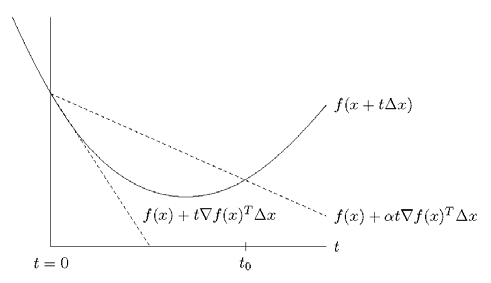
\includegraphics[width=0.5\textwidth]{Pictures/line_search.png}
    \caption{\textit{Backtracking line search.} 
 The lower dashed line shows the linear extrapolation of $f,$ and the upper dashed line has a slope a factor of $\alpha$ smaller. The stopping condition is that $f$ lies below the upper dashed line.}\label{fig:line_search}
\end{figure}
\begin{proposition}\textnormal{\cite[10]{GDandLS}}\label{pf_gd_bt}
Let $f:\mathbb{R}^{n}\longrightarrow\mathbb{R}$ be convex and differentiable. Suppose that $f$ is smooth with Lipschitz constant $L > 0.$ Then gradient descent with backtracking line search satisfies $f(x^{(k)})-f(x^{*}) \leq \frac{||x^{(0)}-x^{*}||^{2}}{2\tau_{min} k},$ where $\tau_{min} = \min\{1,\frac{\beta}{L}\}.$ If $f$ is also strongly convex, then the algorithm satisfies $f(x^{(k)})-f(x^{*}) \leq C^{k}\frac{L}{2}||x^{(0)}-x^{*}||^{2},$ where $C\in(0,1).$
\end{proposition}
For the proof of Proposition \ref{pf_gd_bt}, please refer to the notes by Geoff Gordon and Ryan Tibshirani \cite[10]{GDandLS}. Proposition \ref{pf_gd_bt} allows us to conclude that Algorithm \ref{Pseudo_backtrack} exhibits a running time of $O(1/k)$ for convex objectives and of $O(C^{k})$ for strongly convex objectives. This means that $f(x^{(k)}) \xrightarrow{k\rightarrow\infty} f(x^{*})$ is achieved faster, at exponential rate, for strongly convex objective functions. 